% ---------------------------------------------------------------------
\chapter{Einleitung }
% ---------------------------------------------------------------------

\section{Aufgabenstellung}

Nach der Aufgabenstellung sollen insgesamt 3 Funktionen, nämlich Backup, Restore und upload, erledigt  werden. Die Funktionen sollen mit dem auf Programmiersprache C++ basierenden QT framework implementiert werden. Außerdem sollen die behandelten Dateien oder Dokumente bei Backup und \par Restore laut Anforderungen verschlüsselt und entschlüsselt und in das Internet hochgeladen werden. 
\par Was Backup angeht, handelt es sich um zwei Arten von Backups, nämlich das vollständige und inkrementelle Backup. Das vollständige Backup bezieht sich auf eine ausgewählte ganze Datei und das inkrementelle Backup filtert die bearbeiteten Dateien in einem bestimmten Arbeitsverzeichnis laut einer Zeitspanne heraus. 
\par Die fertige Benutzeroberfläche soll die Schnittstellen bieten, um das exclude-Muster in der Konfigurationsdatei anzuzeigen und zu bearbeiten. Außerdem lassen sich auch noch die Quelladresse und Zieladresse jeweils bei Backup auswählen. Bei Restore wird einfach eine gebackupte Datei in eine Zieladresse gesichert. 
\par Eine Anzeige für die Dateiliste der vorhandenen Backups wird auch angefordert. Auch ist es nötig,  ein paar wichtige Informationen wie zum Beispiel die backupte Dateigröße  auf der Benutzeroberfläche anzuzeigen. 
Darüber hinaus soll die Codes mit Kommandozeilen von Linux ankoppeln, weil das Erzeugnis in Linux-System laufen soll.

\section{Motivation}
Nicht nur die Kenntnisse der Algorithmen und des Rechners, sondern auch der Programmierung sind den Studenten der Fachrichtung Computer Engineering notwendig, um in der Zukunft nach einer guten und geeigneten Arbeitsstelle zu suchen. 
\begin{figure}[h!]
	\centering
	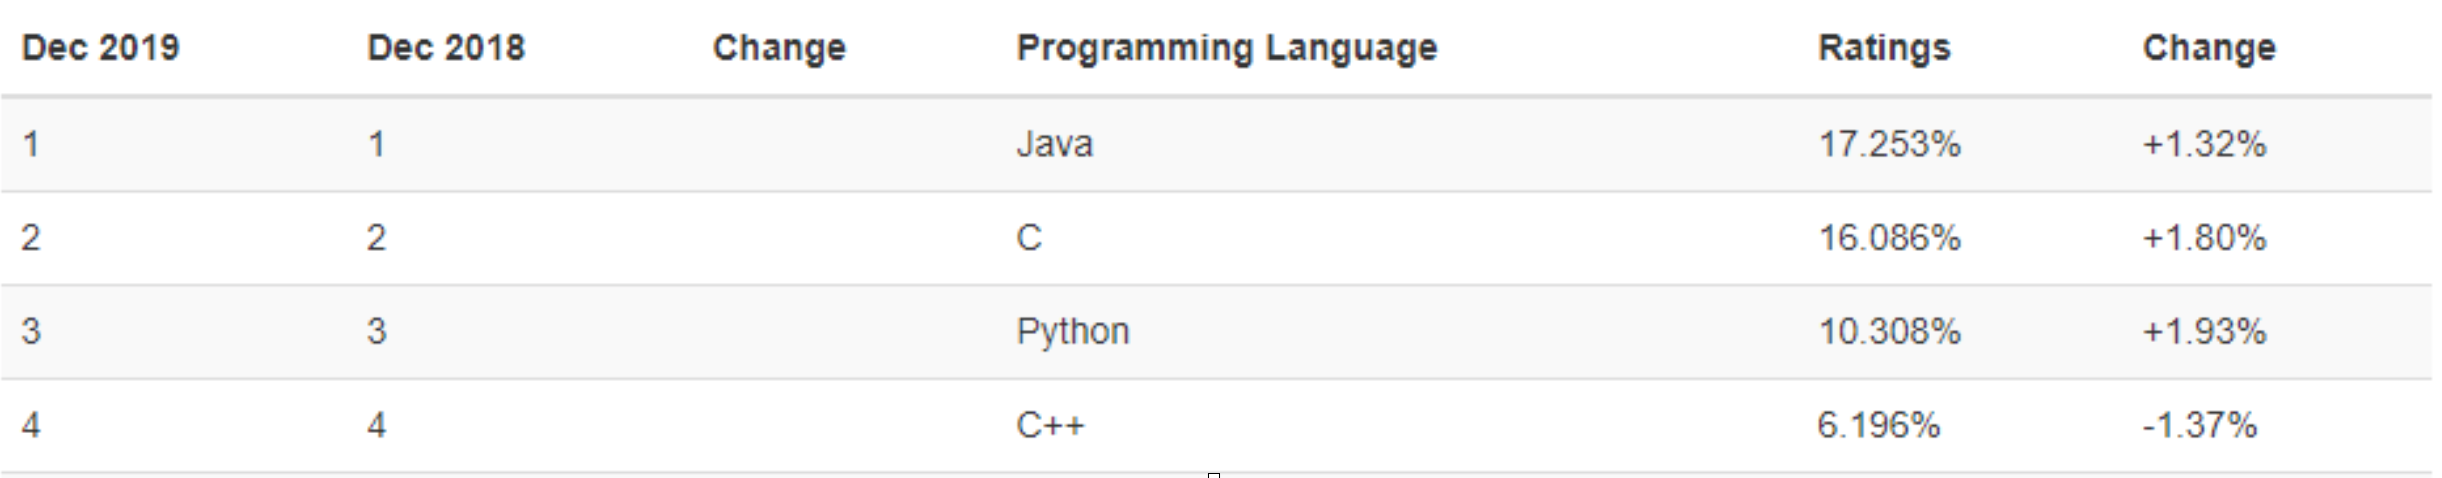
\includegraphics[width=0.8\textwidth]{bilder/rangliste.png}
	\caption{Rangliste der Programmiersprachen in Tobi}
	\label{Abbildung_1}
\end{figure}
\par Bei der kleinen Seminararbeit soll man mit der objektorientierten Programmiersprache C++ auf dem Entwicklungsplattform Qt Creator die Aufgaben erledigen. Zugleich wird mehr und weniger die Erfahrung der Projektentwicklung gesammelt. Auf dem Markt wird in den letzten Jahren die Programmiersprache Python immer mehr populär. Allerdings spiegeln einige Programmiersprachen wie zum Beispiel C++ mit Pointer ein paar Entwicklungsprinzipien des Rechner bei Software und Hardware wider. Deshalb kann mit den Erkenntnissen von C++ auch schneller und leichter andere Programmiersprachen wie Java, Python erfassen.   (s. Abbildung \ref{Abbildung_1}).
\par Außerdem müssen die angeforderten Funktionen in Linux implementiert werden. In Codes werden die Kommandozeilen von Linux integriert.  Somit kann man auch noch während der kleinen Seminararbeit das einen weiten Bereich abdeckende Betriebssystem kennenlernen.


